\documentclass[12pt,a4paper]{article}

% ─── Page Layout ───────────────────────────────────────────────────────────────
\usepackage[a4paper, margin=0.8in, headheight=14pt]{geometry}

% ─── Fonts (XeLaTeX) ───────────────────────────────────────────────────────────
\usepackage{fontspec}
\usepackage{unicode-math}
\setmainfont{TeX Gyre Pagella}
\setmonofont[Scale=0.88]{TeX Gyre Cursor}
\setmathfont{Latin Modern Math}

% ─── Packages ──────────────────────────────────────────────────────────────────
\usepackage{xcolor}
\usepackage{colortbl}
\usepackage{titlesec}
\usepackage{enumitem}
\usepackage{tabularx}
\usepackage{booktabs}
\usepackage{array}
\usepackage{amsmath}
\usepackage{tikz}
\usetikzlibrary{shapes.geometric, arrows.meta, positioning, calc, fit, decorations.pathreplacing}
\usepackage{tcolorbox}
\tcbuselibrary{skins, breakable}
\usepackage{hyperref}
\usepackage{fancyhdr}
\usepackage{graphicx}
\usepackage{microtype}
\hyphenpenalty=10000
\exhyphenpenalty=10000
\sloppy
\usepackage{caption}
\usepackage{setspace}
\usepackage{multirow}
\usepackage{tocloft}

% ─── Q&A helper ────────────────────────────────────────────────────────────────
\newcommand{\Q}[1]{\textbf{#1}\par\noindent\ignorespaces}

% ─── Colour Palette ────────────────────────────────────────────────────────────
\definecolor{myred}{RGB}{196,30,58}
\definecolor{mydark}{RGB}{30,30,50}
\definecolor{mygreen}{RGB}{14,120,80}
\definecolor{myteal}{RGB}{0,130,140}
\definecolor{myamber}{RGB}{180,100,0}
\definecolor{mypurple}{RGB}{100,30,160}
\definecolor{mygray}{RGB}{246,247,249}
\definecolor{mgframe}{RGB}{180,185,200}
\definecolor{watermark}{RGB}{145,150,170}
\definecolor{hdrred}{RGB}{250,232,235}
\definecolor{hdrgreen}{RGB}{220,244,233}
\definecolor{hdrteal}{RGB}{220,242,244}
\definecolor{hdramber}{RGB}{253,242,215}
\definecolor{hdrpurple}{RGB}{238,228,255}
\definecolor{hdrgray}{RGB}{238,240,245}
\definecolor{rowalt}{RGB}{250,251,253}

% ─── Section Formatting ────────────────────────────────────────────────────────
\titleformat{\section}
  {\large\bfseries\color{myred}}{\thesection.}{0.5em}{}
  [\vspace{1pt}{\color{myred}\rule{\linewidth}{0.8pt}}]
\titleformat{\subsection}
  {\normalsize\bfseries\color{myteal}}{\thesubsection}{0.5em}{}
\titlespacing*{\section}{0pt}{18pt}{7pt}
\titlespacing*{\subsection}{0pt}{11pt}{4pt}

% ─── Paragraph ─────────────────────────────────────────────────────────────────
\setlength{\parindent}{0pt}
\setlength{\parskip}{4pt}

% ─── TOC Styling ───────────────────────────────────────────────────────────────
\renewcommand{\cfttoctitlefont}{\large\bfseries\color{myred}}
\renewcommand{\cftaftertoctitle}{\par\noindent{\color{myred}\rule{\linewidth}{0.8pt}}}
\setlength{\cftbeforetoctitleskip}{0pt}
\setlength{\cftaftertoctitleskip}{6pt}
\renewcommand{\cftsecfont}{\normalsize\bfseries\color{mydark}}
\renewcommand{\cftsecpagefont}{\normalsize\bfseries\color{mydark}}
\renewcommand{\cftsecleader}{\cftdotfill{\cftdotsep}}
\setlength{\cftbeforesecskip}{7pt}
\renewcommand{\cftsubsecfont}{\small\color{mydark}}
\renewcommand{\cftsubsecpagefont}{\small\color{mydark}}
\setlength{\cftbeforesubsecskip}{3pt}
\setlength{\cftsubsecindent}{1.4em}

% ─── Table helpers ─────────────────────────────────────────────────────────────
\renewcommand{\arraystretch}{1.45}
\setlength{\tabcolsep}{6pt}
\arrayrulecolor{mydark}
\newcolumntype{B}[1]{>{\small\bfseries\raggedright\arraybackslash}m{#1}}
\newcolumntype{Y}{>{\small\raggedright\arraybackslash}X}
\renewcommand{\tabularxcolumn}[1]{m{#1}}

% ─── Header / Footer ───────────────────────────────────────────────────────────
\pagestyle{fancy}
\fancyhf{}
\fancyhead[L]{\small\color{myred}\textbf{OE-EC604B}\;\color{mydark}--- Operating System}
\fancyhead[R]{\small\color{myteal}\textbf{Module 8 Notes}}
\fancyfoot[C]{\small\color{mydark}\thepage}
\fancyfoot[R]{\small\color{watermark}\textit{\copyright\ Biraj}}
\renewcommand{\headrulewidth}{0.5pt}
\renewcommand{\footrulewidth}{0.3pt}

% ─── Hyperref ──────────────────────────────────────────────────────────────────
\hypersetup{
  colorlinks=true, linkcolor=myteal, urlcolor=myteal,
  pdfauthor={Biraj Sarkar},
  pdftitle={OE-EC604B --- Module 8 Notes}
}

% ─── tcolorbox styles ──────────────────────────────────────────────────────────
\tcbset{
  tikzbox/.style={
    colback=mygray, colframe=mgframe, boxrule=0.6pt, arc=4pt,
    left=8pt, right=8pt, top=6pt, bottom=6pt,
    colbacktitle=mgframe, coltitle=mydark,
    fonttitle=\small\bfseries
  },
  defbox/.style={
    colback=hdrgreen, colframe=mygreen, boxrule=0.8pt, arc=4pt,
    left=9pt, right=9pt, top=6pt, bottom=6pt,
    colbacktitle=mygreen, coltitle=white,
    fonttitle=\small\bfseries
  },
  formulabox/.style={
    colback=hdrteal, colframe=myteal, boxrule=0.8pt, arc=4pt,
    left=9pt, right=9pt, top=7pt, bottom=7pt,
    colbacktitle=myteal, coltitle=white,
    fonttitle=\small\bfseries
  },
  examplebox/.style={
    colback=hdramber, colframe=myamber, boxrule=0.8pt, arc=4pt,
    left=9pt, right=9pt, top=6pt, bottom=6pt,
    colbacktitle=myamber, coltitle=white,
    fonttitle=\small\bfseries
  },
  masonbox/.style={
    colback=hdrpurple, colframe=mypurple, boxrule=0.8pt, arc=4pt,
    left=9pt, right=9pt, top=6pt, bottom=6pt,
    colbacktitle=mypurple, coltitle=white,
    fonttitle=\small\bfseries
  },
  exambox/.style={
    colback=hdrpurple, colframe=mypurple, boxrule=1pt, arc=5pt,
    left=10pt, right=10pt, top=8pt, bottom=8pt,
    colbacktitle=mypurple, coltitle=white,
    fonttitle=\bfseries,
    breakable, title after break={\textbf{Frequently Asked / Viva Questions (contd.)}}}
}
% Make all boxes breakable across pages
\tcbset{breakable}

% ─── TikZ styles ───────────────────────────────────────────────────────────────
\tikzset{
  block/.style={rectangle, draw=myteal, fill=hdrteal,
    text width=2.4cm, align=center, minimum height=0.95cm,
    font=\small, rounded corners=3pt, line width=0.7pt},
  redblock/.style={rectangle, draw=myred, fill=hdrred,
    text width=2.4cm, align=center, minimum height=0.95cm,
    font=\small, rounded corners=3pt, line width=0.7pt},
  greenblock/.style={rectangle, draw=mygreen, fill=hdrgreen,
    text width=2.4cm, align=center, minimum height=0.95cm,
    font=\small, rounded corners=3pt, line width=0.7pt},
  amberblock/.style={rectangle, draw=myamber, fill=hdramber,
    text width=2.4cm, align=center, minimum height=0.95cm,
    font=\small, rounded corners=3pt, line width=0.7pt},
  purpblock/.style={rectangle, draw=mypurple, fill=hdrpurple,
    text width=2.4cm, align=center, minimum height=0.95cm,
    font=\small, rounded corners=3pt, line width=0.7pt},
  sumjunc/.style={circle, draw=myamber, fill=hdramber,
    minimum size=0.62cm, font=\small, line width=0.8pt},
  arrow/.style={-Stealth, thick, color=mydark},
  redarrow/.style={-Stealth, thick, color=myred},
  line/.style={thick, color=mydark}
}

% ═══════════════════════════════════════════════════════════════════════════════
\begin{document}
% ═══════════════════════════════════════════════════════════════════════════════

\begin{center}
  {\LARGE\bfseries\color{myred} OE-EC604B --- Operating System}\\[5pt]
  {\normalsize\color{mydark} Semester VI \quad$\bullet$\quad 3L:0T:0P \quad$\bullet$\quad 3 Credits}\\[3pt]
  {\normalsize\color{myteal}\textbf{Module 8 Exam Notes: File Systems}}\\[3pt]
  {\small\color{mydark} CGEC \;$|$\; B.Tech ECE (2023--27) \;$|$\; \textit{Biraj Sarkar}}
\end{center}
\vspace{2pt}
\noindent{\color{myred}\rule{\linewidth}{1.5pt}}
\vspace{2pt}

\hypersetup{linkcolor=mydark}
\tableofcontents
\hypersetup{linkcolor=myteal}
\newpage

% ===============================================================================
\section{File and Directory Concepts}
% ===============================================================================

The file system provides the online storage and access mechanism for both data and programs of the operating system.

\subsection{File Concepts \& Access Mechanisms}
\begin{itemize}[leftmargin=*, itemsep=3pt]
  \item \textbf{File Concept:} A file is a named collection of related information that is recorded on secondary storage.
  \item \textbf{Access Methods:}
  \begin{itemize}[leftmargin=*, itemsep=2.5pt, topsep=0pt]
    \item \textbf{Sequential Access:} Information is processed in order, one record after another (e.g., tape storage).
    \item \textbf{Direct (Random) Access:} A file is viewed as a numbered sequence of blocks. The program can read/write any block instantly in any order (e.g., database queries on disk).
    \item \textbf{Indexed Access:} An index table is built containing pointers to various blocks. The program searches the index first to retrieve records.
    \end{itemize}
  \end{itemize}

\subsection{Directory Structures}
A directory is a container that organizes files. Common topologies:
\begin{itemize}[leftmargin=*, itemsep=3pt]
  \item \textbf{Single-Level Directory:} All files are in a single directory. \textbf{Problems:} Naming collisions, organization issues.
  \item \textbf{Two-Level Directory:} Each user gets a private User File Directory (UFD) nested under a Master File Directory (MFD).
  \item \textbf{Tree-Structured Directory:} Users can create subdirectories and organize files hierarchically. The most common structure.
\end{itemize}

\begin{tcolorbox}[tikzbox, title={Tree-Structured Directory Tree}]
\centering
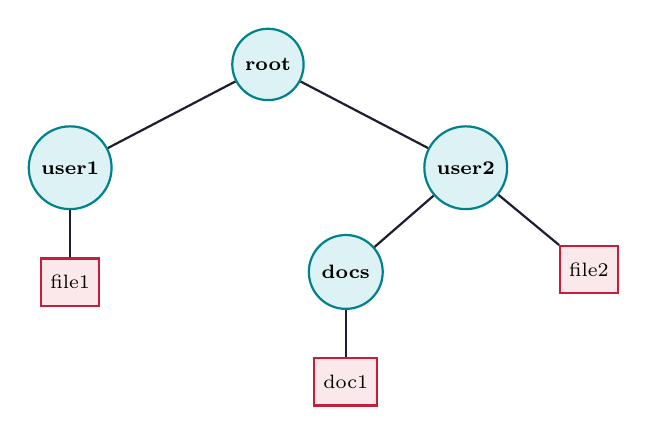
\begin{tikzpicture}[node distance=0.8cm, thick, font=\small,
  dir/.style={circle, draw=myteal, fill=hdrteal, minimum size=0.8cm, font=\scriptsize\bfseries},
  file/.style={rectangle, draw=myred, fill=hdrred, minimum size=0.6cm, font=\scriptsize}]
  \node[dir] (root) {root};
  \node[dir, below left=0.6cm and 1.8cm of root] (user1) {user1};
  \node[dir, below right=0.6cm and 1.8cm of root] (user2) {user2};
  
  \node[file, below=0.6cm of user1] (f1) {file1};
  \node[dir, below left=0.6cm and 0.8cm of user2] (sub) {docs};
  \node[file, below right=0.6cm and 0.8cm of user2] (f2) {file2};
  \node[file, below=0.6cm of sub] (f3) {doc1};

  \draw[line] (root) -- (user1);
  \draw[line] (root) -- (user2);
  \draw[line] (user1) -- (f1);
  \draw[line] (user2) -- (sub);
  \draw[line] (user2) -- (f2);
  \draw[line] (sub) -- (f3);
\end{tikzpicture}
\tcbset{breakable}
\end{tcolorbox}

% ===============================================================================
\section{File System Implementation and Allocation Methods}
% ===============================================================================

To store files on disk, the OS must map logical file blocks to physical disk sectors. There are three traditional allocation methods:

\subsection{1. Contiguous Allocation}
\begin{itemize}[leftmargin=*, itemsep=3pt]
  \item \textbf{Working:} Each file occupies a contiguous set of blocks on the disk.
  \item \textbf{Advantages:} Fast sequential read/write operations because the disk head does not need to move. Easy direct access.
  \item \textbf{Disadvantages:} Prone to \textbf{external fragmentation}. Hard to grow a file dynamically if adjacent blocks are already allocated.
\end{itemize}

\subsection{2. Linked Allocation}
\begin{itemize}[leftmargin=*, itemsep=3pt]
  \item \textbf{Working:} Each file is a linked list of disk blocks. Directory contains a pointer to the first and last blocks of the file. Each block contains a pointer to the next block.
  \item \textbf{Advantages:} No external fragmentation. Files can grow indefinitely.
  \item \textbf{Disadvantages:} Slow random (direct) access (must traverse links sequentially from block 1). Pointers consume storage space. If a pointer gets corrupted, the rest of the file is lost.
  \item \textbf{FAT (File Allocation Table):} A variation of linked allocation. Pointers are stored in a centralized table at the beginning of the volume, caching entries for faster lookup.
\end{itemize}

\subsection{3. Indexed Allocation}
\begin{itemize}[leftmargin=*, itemsep=3pt]
  \item \textbf{Working:} Each file has its own \textbf{index block}, which contains an array of pointers to all its physical data blocks.
  \item \textbf{Advantages:} Supports direct access without traversing lists. No external fragmentation.
  \item \textbf{Disadvantages:} Index block overhead --- wastes space for very small files. If a file grows too large, a single index block is insufficient. (Resolved using linked index blocks, multilevel indexing, or UNIX indirect blocks).
\end{itemize}

% ===============================================================================
\section{Free Space Management}
% ===============================================================================

To allocate blocks, the OS tracks all free disk blocks using one of two common methods:
1. \textbf{Bit Vector (Bit Map):} An array of bits where each bit corresponds to a disk block (0 = allocated, 1 = free). \textbf{Advantages:} Fast, easy to find consecutive blocks. \textbf{Disadvantages:} Must be kept in RAM, consumes space for large disks.
2. \textbf{Linked List:} All free blocks are linked together. Directory keeps a pointer to the first free block. \textbf{Advantages:} Minimal space overhead. \textbf{Disadvantages:} Slow to traverse; hard to find contiguous free blocks.

\newpage
% ===============================================================================
% MANDATORY QUICK REVISION PAGE
% ===============================================================================
\begin{center}
  {\large\bfseries\color{myred} Quick Revision --- Module 8}\\[3pt]
  {\small\color{mydark} File Systems $|$ OE-EC604B}
\end{center}
\noindent{\color{myred}\rule{\linewidth}{1.2pt}}
\vspace{4pt}

\begin{tcolorbox}[formulabox, title={\textbf{File Allocation Calculations}}]
Let block size = $1\,\text{KB}$. Pointer size = $4\,\text{Bytes}$.
\begin{itemize}[leftmargin=*, itemsep=3pt]
  \item \textbf{Single Index Block Limit:} An index block can hold $1\,\text{KB} / 4\,\text{B} = 256$ pointers. Max file size = $256 \times 1\,\text{KB} = 256\,\text{KB}$.
  \item \textbf{Two-Level Indexing Limit:} Primary index block points to 256 secondary index blocks. Max file size = $256 \times 256 \times 1\,\text{KB} = 64\,\text{MB}$.
\end{itemize}
\end{tcolorbox}

\begin{tcolorbox}[defbox, title={\textbf{One-Line Definitions}}]
\begin{itemize}[leftmargin=*, itemsep=2.5pt, topsep=0pt]
  \item \textbf{File:} A named logical collection of related records stored on secondary storage.
  \item \textbf{Sequential Access:} Access method where data is read in sequence from beginning to end.
  \item \textbf{Direct Access:} Random block access where records are accessed directly by block index.
  \item \textbf{Contiguous Allocation:} Allocation method where file blocks are saved in consecutive disk sectors.
  \item \textbf{Linked Allocation:} Allocation method where blocks are linked via pointers in a list structure.
  \item \textbf{FAT:} File Allocation Table; centralized directory indexing system caching linked pointers.
  \item \textbf{Indexed Allocation:} Allocation method where all block pointers are collected in an index block.
  \item \textbf{Bit Vector:} Binary sequence where each bit represents the free/allocated state of a disk block.
\end{itemize}
\end{tcolorbox}

\begin{tcolorbox}[exambox, title={\textbf{Frequently Asked / Viva Questions}}]
\begin{enumerate}[topsep=0pt, label=\textbf{Q\arabic*.}, itemsep=5pt]
  \item \Q{Compare Contiguous, Linked, and Indexed file allocation methods.}
    Contiguous is fast, supports direct access, but suffers from external fragmentation and file-growth limitations. Linked eliminates fragmentation and allows files to grow easily but has slow random access and pointer overhead. Indexed supports direct access and file growth with no fragmentation, but has index block space overhead.
  \item \Q{Explain the FAT (File Allocation Table) file system structure.}
    FAT is a variation of linked allocation. It extracts all block pointers from the data blocks and stores them in a centralized table at the beginning of the partition. The directory entry contains the starting block number, and the table is indexed by block numbers to find subsequent blocks.
  \item \Q{What is an index block in file system implementation? What happens if a file exceeds its capacity?}
    An index block contains an array of disk block addresses allocated to a file. If a file exceeds the index block capacity, the OS uses: 1. Linked scheme (linking multiple index blocks). 2. Multilevel indexing (an index block containing pointers to other index blocks). 3. Combined scheme (like UNIX inodes).
  \item \Q{Describe free space management using a Bit Vector. Calculate the size of a bit map for a 200 GB disk with 4 KB blocks.}
    A bit vector uses 1 bit for each disk block: 1 means free, 0 means allocated.
    \textbf{Total Blocks} = $200\,\text{GB} / 4\,\text{KB} = (200 \times 10^9) / (4 \times 10^3) = 50 \times 10^6$ blocks.\par
    \textbf{Map Size} = $50 \times 10^6$ bits $\approx 6.25\,\text{MB}$ of storage.
  \item \Q{Explain the difference between sequential and direct file access mechanisms.}
    Sequential access processes records one after another from the beginning, moving a read pointer sequentially. Direct access allows reading/writing blocks in any arbitrary order by specifying the relative block number directly.
  \item \Q{What are the advantages of a tree-structured directory over a single-level directory?}
    A tree-structured directory allows users to create nested subdirectories to organize files logically, preventing naming conflicts and enabling file organization, sharing, and access control.
  \item \Q{Explain the implementation issues of contiguous allocation.}
    Finding space for a new file requires executing dynamic allocation algorithms (first-fit, best-fit), which leads to external fragmentation. Also, if a file grows, it may collide with an adjacent allocated file, requiring compaction.
  \item \Q{Why does linked allocation suffer from reliability issues?}
    Because the blocks are scattered across the disk, and each block contains a pointer to the next. If a single sector gets corrupted, the pointer is lost, rendering all subsequent blocks inaccessible.
  \item \Q{What is the purpose of directory mounting?}
    Mounting allows the OS to attach multiple physical file systems on different storage devices (hard disks, USB drives) into a single, unified logical directory tree.
  \item \Q{How does the OS optimize directory lookup speed?}
    By using hash tables or B-trees instead of linear lists to store directory entries, reducing lookup times from $O(N)$ to $O(1)$ or $O(\log N)$.
\end{enumerate}
\end{tcolorbox}

\begin{tcolorbox}[tikzbox, title={File Allocation Methods Comparison}]
\renewcommand{\arraystretch}{1.4}
\par\noindent
\begin{tabularx}{\linewidth}{|B{2.2cm}|>{\small\centering\arraybackslash}X|>{\small\centering\arraybackslash}X|>{\small\centering\arraybackslash}X|}
\hline
\textbf{Feature} & \textbf{\color{myred}Contiguous} & \textbf{\color{myteal}Linked} & \textbf{\color{myamber}Indexed} \\
\hline
\textbf{Direct Access} & Excellent & Very Poor (linear traversal) & Excellent \\
\hline
\textbf{External Frag.} & Yes & None & None \\
\hline
\textbf{Storage Efficiency} & High & Moderate (pointer overhead) & Low for small files \\
\hline
\textbf{File Growth} & Hard (contiguous block) & Easy & Easy \\
\hline
\end{tabularx}
\end{tcolorbox}

\end{document}
